\documentclass[sigconf,nonacm]{acmart}

% ---- Packages ----
\usepackage{booktabs,graphicx}
\usepackage{amsmath}
\usepackage{makecell}
\usepackage{tikz}
\usepackage{placeins}
\usetikzlibrary{positioning,arrows.meta,calc}
\usepackage[capitalize]{cleveref}
\usepackage{microtype}                 % char protrusion + font expansion: fixes text spilling past the margin
\setlength{\emergencystretch}{3em}     % allow extra glue on hard lines so nothing overflows the text block
\raggedbottom
\setlength{\textfloatsep}{9pt plus 2pt minus 2pt}
\setlength{\dbltextfloatsep}{9pt plus 2pt minus 2pt}
\setlength{\floatsep}{8pt plus 2pt minus 2pt}
\setlength{\dblfloatsep}{8pt plus 2pt minus 2pt}
\setlength{\intextsep}{8pt plus 2pt minus 2pt}
\setlength{\abovecaptionskip}{5pt}
\setlength{\belowcaptionskip}{0pt}
\renewcommand{\topfraction}{0.95}
\renewcommand{\dbltopfraction}{0.95}
\renewcommand{\textfraction}{0.05}
\renewcommand{\floatpagefraction}{0.82}
\renewcommand{\dblfloatpagefraction}{0.82}

\definecolor{stagebluefill}{HTML}{EAF2FF}
\definecolor{stageblueedge}{HTML}{2563EB}
\definecolor{stagepurplefill}{HTML}{F1EBFF}
\definecolor{stagepurpleedge}{HTML}{7C3AED}
\definecolor{stageredfill}{HTML}{FDECEC}
\definecolor{stagerededge}{HTML}{DC2626}
\definecolor{stageorangefill}{HTML}{FFF1E8}
\definecolor{stageorangeedge}{HTML}{EA580C}
\definecolor{stagegoldfill}{HTML}{FFF7D6}
\definecolor{stagegoldedge}{HTML}{CA8A04}
\definecolor{stagegreenfill}{HTML}{EAF7EE}
\definecolor{stagegreenedge}{HTML}{15803D}
\definecolor{stageslatefill}{HTML}{F8FAFC}
\definecolor{stageslateedge}{HTML}{475569}

% ---- acmart housekeeping (nonacm) ----
\settopmatter{printacmref=false}
\setcopyright{none}
\pagestyle{plain}
\graphicspath{{figures/}}
\input{results_macros_gen}

\begin{document}

% ---- Title / authors ----
\title{The Benchmark Chooses the Winner: Measuring Fine-Tuning Specialization Across Safety-Guard Benchmarks}

\author{Reza Rahimi}
\email{reza.rahimi@jazzx.ai}
\affiliation{%
  \institution{JazzX AI}
  \city{Los Altos}
  \state{CA}
  \country{USA}
}

\begin{abstract}
Small language models are increasingly adapted into binary prompt-safety guards, but improvement on benchmark sources represented during training does not establish transfer to other datasets. We retrospectively analyze a fixed legacy run that compares four untuned checkpoints (1.5B--4B parameters) with five LoRA-SFT seeds per checkpoint. The training rows, semantic classification instruction, LoRA capacity, and evaluation rows are fixed; rendered chat serialization is model-specific. We separate represented-source tests from four dataset-held-out transfer benchmarks and report macro average precision (AP), per-source effects, and calibration-only operating points.

The fixed-panel base-to-SFT changes are $\RepDelta$ in represented-source macro AP (95\% two-sided paired-bootstrap interval $[\RepCILower,\RepCIUpper]$) and $\TransferDelta$ in transfer macro AP ($[\TransferCILower,\TransferCIUpper]$). Transfer is heterogeneous across checkpoints, but every leave-one-checkpoint-out and leave-one-transfer-benchmark-out sensitivity estimate remains negative. At calibration-targeted thresholds, benchmark-macro transfer FPR rises from \TransferBaseFPRPct\% (base) to \TransferSFTFPRPct\% (SFT), while pooled-negative FPR rises from \TransferBasePooledFPRPct\% to \TransferSFTPooledFPRPct\%; HarmBench recall falls from \HarmBenchBaseRecallPct\% to \HarmBenchSFTRecallPct\%.

Prior work has established policy overfitting, calibration sensitivity, and safety degradation after fine-tuning. Our contribution is narrower: a same-checkpoint, same-training-manifest characterization of how compact prompt guards move across benchmark sources. Conditional on these four checkpoints and seven fixed AP datasets, the estimates are consistent with in-source specialization, not a general moderation upgrade. Because the committed scores predate the strengthened provenance and lock contract released with this paper, we treat the result as estimation-only and identify the clean rerun required for confirmatory use.
\end{abstract}

\maketitle

\section{Introduction}
\label{sec:intro}

Teams increasingly convert a general instruction model into a safety guard with a short parameter-efficient fine-tune, then report the adapted guard's score on a public benchmark suite. A post-adaptation leaderboard number, however, hides the quantity a practitioner actually needs: what changed relative to the same checkpoint before adaptation, and whether that change transfers to datasets not represented during training. Because an adapted guard is often compared only against \emph{other} models, a gain on represented benchmark sources can be mistaken for broader discrimination or policy agreement.

This paper asks one question: \emph{what does LoRA-SFT add beyond the untuned base model, and does that gain transfer to evaluation datasets whose rows were not used for SFT?} We retrospectively analyze a controlled, same-checkpoint, same-training-manifest, multi-seed run on a fixed four-checkpoint panel (Qwen2.5-1.5B, SmolLM2-1.7B, SmolLM3-3B, Qwen3-4B) and one frozen LoRA-SFT recipe, comparing every adapted guard against its own untuned base across two evaluation regimes: benchmark sources \emph{represented} during training and \emph{dataset-held-out} benchmarks whose rows were withheld from SFT.

We organize the analysis around the following deliberately panel-limited question.

\begin{quote}
For a fixed four-checkpoint panel and one frozen LoRA-SFT recipe, does guard adaptation change discrimination differently on represented-source and dataset-held-out tests?
\end{quote}

The design and analysis were not publicly preregistered, and the committed run is analyzed retrospectively. We therefore report estimates, intervals, heterogeneity, and sensitivity checks without confirmatory rejection language.

\paragraph{Scope.} The study is deliberately narrow: English input-prompt classification, binary safe/unsafe decision-token scoring, small instruction models from 1.5B to 4B parameters, one fixed LoRA-SFT recipe, three represented-source datasets, four dataset-held-out transfer benchmarks, two single-class stress sets, and a fixed, purposively chosen four-checkpoint panel. It is not a guardrail leaderboard, an objective comparison, an ensembling study, a fairness audit, a frontier-API parity or latency study, or a domain-compliance case study; those questions --- including the mortgage-compliance case study --- are out of scope here and are treated in separate work. Response, tool-call, and full-dialogue moderation, arbitrary unseen policies, production traffic, and universal claims about fine-tuning are likewise out of scope.

\subsection{Contributions}
\label{sec:contributions}

The paper makes exactly three contributions.

\begin{itemize}
  \item \textbf{Controlled base-to-guard comparison.} For each checkpoint, we compare the untuned base with five SFT adapters on identical evaluation rows, semantic instructions, score definitions, and metrics, isolating the within-checkpoint change in this executed run.
  \item \textbf{Fixed-panel transfer characterization.} We estimate represented-source and dataset-held-out changes separately, report per-base and per-benchmark heterogeneity, and restrict every conclusion to the named four-checkpoint panel and frozen recipe.
  \item \textbf{Auditable measurement package.} We release a text-free public manifest index, source revisions, content hashes, seed-level results, keyed scores, paired intervals, generated tables and figures, and an executable cached-analysis path. Raw third-party rows remain local according to their licenses.
\end{itemize}

Operating-point evaluation (\Cref{subsec:operating-point}) is \emph{supporting methodology, not a contribution}: it is a secondary deployment diagnostic and does not provide a distribution-free production guarantee.

\subsection{Research questions}
\label{sec:rqs}

The single question above is operationalized as four research questions.

\begin{description}
  \item[RQ1 (represented-source effect).] For the fixed four-checkpoint panel, how does a common LoRA-SFT recipe change macro average precision on benchmark sources represented during training?
  \item[RQ2 (benchmark-transfer effect).] How does the same adaptation change macro average precision on dataset-held-out transfer benchmarks?
  \item[RQ3 (heterogeneity).] Are the represented-source and transfer changes stable across checkpoints and evaluation datasets, or are they concentrated in particular bases and benchmarks?
  \item[RQ4 (deployment sensitivity).] What TPR/FPR trade-off do the base and SFT systems realize when thresholds are selected on calibration data at a nominal 5\% pooled-negative FPR target?
\end{description}

RQ4 is descriptive and secondary: it does not provide a distribution-free production guarantee, and failure to obtain a feasible threshold under the prespecified bound is a reportable outcome rather than grounds for selecting a threshold on test data.

\section{Related Work}
\label{sec:related}

\textbf{Small-LLM guard classifiers.} A growing family of purpose-built classifiers screens prompts and responses for LLM pipelines --- Llama Guard \cite{inan2023llamaguard,meta2024llamaguard3_1b}, ShieldGemma \cite{zeng2024shieldgemma}, Granite Guardian \cite{padhi2024graniteguardian}, WildGuard \cite{han2024wildguard}, and LoRA-Guard \cite{elesedy2024loraguard} --- typically framing moderation as supervised classification that emits a verdict token or score. Efficiency-oriented work argues that small, cheap classifiers can serve as practical guards \cite{majhi2025gpuguard}, and GuardBench shows that a general instruction-tuned model can rival guard-specific fine-tunes on a large suite \cite{bassani2024guardbench}. Our guard formulation is deliberately minimal --- a single-token \{safe, unsafe\} logprob head read in one forward pass, LoRA-tuned from a compact instruction base \cite{bakouch2025smollm3,hu2021lora} --- because the object of study is the \emph{before-versus-after} effect of adaptation, not a new architecture.

\textbf{Fine-tuning degradation and benchmark/policy transfer.} Prior work establishes that fine-tuning can degrade a model's safety behavior and analyzes when this happens through alignment/fine-tuning similarity \cite{hsiung2025guardrails}. Policy-overfitting and unseen-policy adaptation are studied directly by augmented policy training for domain-generalizable guardrails \cite{liu2026domaingeneralizable}; surface-heuristic reliance and robustness failures further limit out-of-distribution claims \cite{li2026surfaceheuristics,bassani2025robustness}. Specialized-domain moderation is evaluated by expert-annotated benchmarks such as ExpGuard \cite{expguard2026}. Detector rankings are regime-dependent \cite{akinrele2026regime}, and fine-tuning objectives themselves shape safety and robustness \cite{vennemeyer2026objective}. We therefore claim only a paired base-to-SFT characterization on a fixed panel, separated into represented and dataset-held-out sources.

\textbf{Calibration and operating points.} Guard scores require calibration to be read as probabilities or thresholds; temperature scaling \cite{guo2017calibration} and guard-specific calibration analyses \cite{liu2025calibration} are standard, while FlexGuard studies continuous risk scoring and cross-strictness behavior \cite{flexguard2026}. Calibrated ensembles can mitigate accuracy trade-offs under distribution shift \cite{kumar2022calibrated}. We use calibration only as a secondary operating-point diagnostic (\Cref{subsec:operating-point}) fit on held-back calibration rows, never on transfer or stress data, and we do not propose a new calibration method.

\textbf{Novelty boundary.} Unlike work proposing new policy augmentation, calibration, or preservation objectives, we isolate the before-versus-after effect of a common SFT guard recipe on the same compact checkpoints and report represented-source and dataset-held-out changes separately. We do not claim a new metric, calibration algorithm, preservation loss, preference-learning method, ensemble, compliance architecture, or theorem. The defensible novelty is a controlled, same-checkpoint, same-training-manifest, multi-seed estimate of how compact binary prompt guards move between represented-source discrimination and dataset-held-out benchmark transfer.

\section{Controlled Study Design}
\label{sec:design}

\Cref{fig:design} summarizes the intended pipeline: pinned source snapshots are compiled into manifests, audited, and locked; four bases are each adapted with five SFT seeds; the base and adapted guards are scored on represented-source, transfer, and stress manifests; and paired deltas feed estimation and sensitivity analyses. Training does not read evaluation rows. Manifest construction, audit, threshold fitting on calibration data, and analysis necessarily read their corresponding labels. The committed score table is from a legacy contract; the corrected builder and lock verifier require a new GPU run before claims can be called clean-run results.

\begin{figure}[t]
\centering
\resizebox{\columnwidth}{!}{%
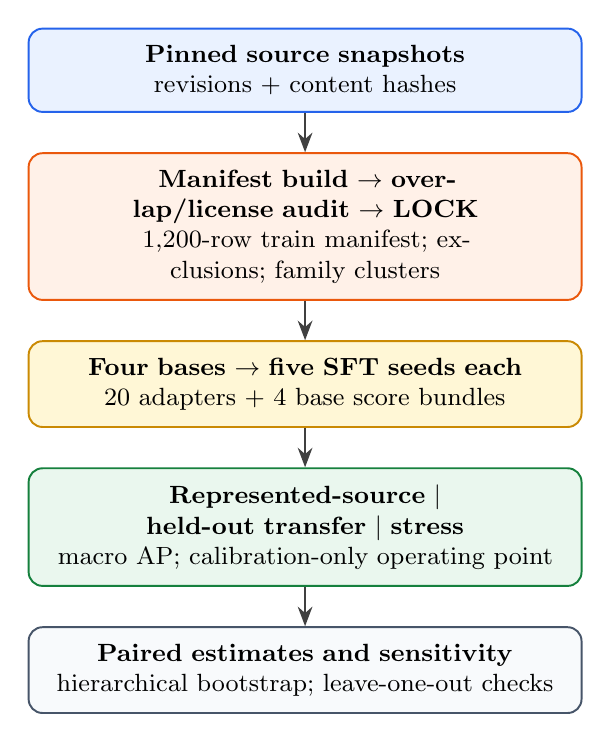
\begin{tikzpicture}[
  >=Stealth,
  node distance=5mm,
  stage/.style={draw, rounded corners=5pt, line width=0.7pt, align=center, inner sep=6pt, font=\small, text width=66mm},
  flow/.style={->, line width=0.9pt, draw=black!75}
]
  \node[stage, fill=stagebluefill, draw=stageblueedge] (src) {\textbf{Pinned source snapshots}\\ revisions $+$ content hashes};
  \node[stage, fill=stageorangefill, draw=stageorangeedge, below=of src] (lock) {\textbf{Manifest build $\to$ overlap/license audit $\to$ LOCK}\\ 1{,}200-row train manifest; exclusions; family clusters};
  \node[stage, fill=stagegoldfill, draw=stagegoldedge, below=of lock] (train) {\textbf{Four bases $\to$ five SFT seeds each}\\ 20 adapters $+$ 4 base score bundles};
  \node[stage, fill=stagegreenfill, draw=stagegreenedge, below=of train] (eval) {\textbf{Represented-source $\mid$ held-out transfer $\mid$ stress}\\ macro AP; calibration-only operating point};
  \node[stage, fill=stageslatefill, draw=stageslateedge, below=of eval] (gate) {\textbf{Paired estimates and sensitivity}\\ hierarchical bootstrap; leave-one-out checks};
  \draw[flow] (src) -- (lock);
  \draw[flow] (lock) -- (train);
  \draw[flow] (train) -- (eval);
  \draw[flow] (eval) -- (gate);
\end{tikzpicture}%
}
\caption{Study design for a clean rerun. Source snapshots are frozen and audited before training; evaluation manifests are scored only after all twenty adapters and four base bundles exist. Paired base-versus-SFT deltas drive estimation and sensitivity analyses.}
\Description{Five connected stages: pinned source snapshots; manifest construction, audit, and lock; four base models with five SFT seeds each; represented-source, transfer, and stress evaluation; and paired estimation with sensitivity checks.}
\label{fig:design}
\end{figure}

\subsection{Prompt-safety task and label mapping}
\label{subsec:task}

The guard is a binary classifier that emits a single-token verdict, \texttt{safe} or \texttt{unsafe}. A prompt is \texttt{unsafe} when the source annotation maps it to harmful, jailbreak, prompt-injection, or policy-violating content; a labeled attempt need not have succeeded against a target model. Each source's native label is mapped by a fixed rule: ToxicChat \cite{lin2023toxicchat} \texttt{toxicity}$=1\!\to\!$unsafe; \texttt{deepset/prompt-injections} \texttt{label}$=1\!\to\!$unsafe; \texttt{jailbreak-classification} \texttt{type} beginning \emph{jailbreak}$\to\!$unsafe; JailbreakBench \cite{chao2024jailbreakbench} harmful/benign splits; XSTest \cite{rottger2024xstest} contrast prompts$\to\!$unsafe; WildGuardTest \cite{han2024wildguard} \texttt{prompt\_harm\_label}; WildJailbreak \cite{jiang2024wildteaming} integer label; OR-Bench-Hard \cite{cui2024orbench} benign portion (safe); and HarmBench \cite{mazeika2024harmbench} behaviors (unsafe). These heterogeneous mappings do not define one universal moderation policy.

\subsection{Guard formulation: a single-token logprob head}
\label{subsec:guard}

The guard treats safety classification as a single next-token prediction. A prompt $x$ is wrapped in one versioned instruction template shared across every base and seed, and the model is asked for a one-word verdict. Rather than sampling text, we read the last-position logits and restrict attention to the two verdict tokens. Let $z_{\text{safe}}(x,t)$ and $z_{\text{unsafe}}(x,t)$ be those logits at the final prompt position $t$. The stored canonical score is the logit difference
\begin{equation}
\label{eq:score}
s(x) = z_{\text{unsafe}}(x,t) - z_{\text{safe}}(x,t),
\end{equation}
and the derived probability is the two-way softmax
\begin{equation}
\label{eq:prob}
p(\text{unsafe}\mid x) = \frac{\exp(z_{\text{unsafe}})}{\exp(z_{\text{safe}}) + \exp(z_{\text{unsafe}})}.
\end{equation}
Raw \texttt{safe}/\texttt{unsafe} logits are the canonical stored values; probabilities and temperature-scaled values are derived from them. Generated verdict text is never used as the primary score. For each checkpoint we verify that the decision tokens are distinct single tokens under a fixed convention (leading-space \texttt{" safe"}/\texttt{" unsafe"} first, no-leading-space fallback), and store token IDs, token strings, truncation state, and scored/original token counts. The semantic system instruction is shared, but model-specific chat templates produce three distinct rendered-template hashes across the four checkpoints. The corrected runner preserves the classification instruction under truncation; the legacy scores include left-truncated examples, quantified in \Cref{sec:limitations}.

\subsection{Training manifest and exclusions}
\label{subsec:manifest}

Training reads one frozen 1{,}200-row manifest and never resamples live datasets during a run. It draws \textbf{400 rows each} from three represented sources --- ToxicChat, Prompt-Injections, and Jailbreak-Classification --- with \textbf{200 safe and 200 unsafe} rows per source, selected by a SHA-256 hash rank salted with \texttt{data\_seed} and shared as one fixed row order across every checkpoint and training seed. At effective batch size 4, 1{,}200 rows produce exactly 300 optimizer updates for one complete exposure.

\textbf{BeaverTails and OR-Bench are excluded from training.} BeaverTails' \texttt{is\_safe} annotation labels the prompt--response interaction rather than the prompt alone, and OR-Bench is reserved for the benign stress set and shares an evaluation family; including either would confound the prompt-only, dataset-held-out design. The study uses the non-commercial academic data branch (ToxicChat is CC BY-NC 4.0), so any released adapter is marked non-commercial. We do not redistribute third-party raw text; the release provides pinned identifiers, revisions, and content hashes.

\textbf{Decontamination audit.} The corrected builder preserves authoritative upstream conversation/pair/scenario identifiers, adds deterministic character 5-gram MinHash edges, constructs connected components before splitting represented-source calibration and ID rows, and fails closed if any family crosses train/evaluation or calibration/any reported test or stress boundary. It also hard-asserts source exclusions, exact/conflicting-label overlap, source revisions, content hashes, selection provenance, and near-duplicate dispositions. The historical audit associated with the committed scores reported zero exact and conflicting-label train/evaluation overlaps, but its family keys failed to join 36 JailbreakBench matched-index pairs and 58 XSTest safe/unsafe pairs; two represented-source families also crossed calibration and ID. Its six approximate train/evaluation pairs at the 0.80 sensitivity threshold were reported rather than adjudicated. Consequently, the historical family bootstrap and operating-point split are descriptive artifacts; the repaired family graph must be used in a clean rerun.

\begin{table*}[t]
\centering
\small
\caption{Data sources and roles in the legacy score artifact. Train counts are 400 per source (200 safe / 200 unsafe). Dataset revisions, content hashes, redistribution fields, and license evidence are recorded in the text-free public manifest index. WildGuardTest and WildJailbreak counts are legacy seed-7 cohorts; the corrected builder defaults to pinned-source hash ranking, so a clean rerun will produce different cohorts.}
\label{tab:data-roles}
\begin{tabular}{lllll}
\toprule
Source (Hugging Face) & Native label origin & Role & Count (target) & License \\
\midrule
\texttt{lmsys/toxic-chat} & prompt toxicity & train $+$ calibration/ID & 400 train (200:200) & CC BY-NC 4.0 \\
\texttt{deepset/prompt-injections} & prompt injection & train $+$ calibration/ID & 400 train (200:200) & metadata conflict$^\dagger$ \\
\texttt{jackhhao/jailbreak-classification} & prompt jailbreak & train $+$ calibration/ID & 400 train (200:200) & Apache-2.0 \\
\midrule
\texttt{JailbreakBench/JBB-Behaviors} & harmful/benign split & transfer (test only) & 120 (60:60) & MIT \\
\texttt{natolambert/xstest-v2-copy} & contrast prompt & transfer (test only) & 240 (120:120) & CC BY 4.0 \\
\texttt{allenai/wildguardmix} & prompt harm label & transfer (test only) & 800 (400:400) & ODC-BY $+$ AI2 \\
\texttt{allenai/wildjailbreak} & adversarial label & transfer (test only) & 420 (210:210) & ODC-BY $+$ AI2 \\
\midrule
\texttt{bench-llm/or-bench} (hard-1k) & benign over-refusal & stress: benign FPR only & 400 (0:400) & CC BY 4.0 \\
\texttt{walledai/HarmBench} & harmful & stress: recall only & 200 (200:0) & MIT \\
\bottomrule
\end{tabular}
\vspace{2pt}\parbox{0.97\textwidth}{\footnotesize $^\dagger$At the pinned Prompt-Injections revision, top-level card metadata says Apache-2.0 while nested dataset metadata says CC BY 4.0; the public index records the conflict rather than silently choosing one.}
\end{table*}

\subsection{Model panel and frozen SFT recipe}
\label{subsec:panel}

The estimand is a fixed, purposively chosen four-checkpoint panel; we do not bootstrap model identities or infer over model families. All checkpoints, revisions, and the LoRA-SFT recipe are in \Cref{tab:panel-recipe}. Each base is adapted with five training seeds (42--46) sharing data-order seed 42, giving 20 adapters; four untuned bases are scored once and reused ($4+20=24$ model bundles). The executed recipe uses completion-only loss on the verdict and appended EOS tokens, LoRA $r{=}32$, $\alpha{=}64$, dropout $0.05$ on q/k/v/o/gate/up/down projections, 300 steps, learning rate $2\times10^{-4}$ with cosine schedule and 0.03 warmup, effective batch 4, and maximum sequence length 1{,}024. The historical tokenizer left-truncated overlength inputs; the corrected runner preserves the system instruction and records the truncation strategy.

\begin{table*}[t]
\centering
\small
\caption{Fixed model panel and executed LoRA-SFT recipe. Revisions are pinned and decision tokens are verified as distinct single tokens. Training-token and wall-time values are medians across five legacy runs; run metadata also records the A100 device, peak memory, and per-run timing, but not every software/driver field required by the new contract.}
\label{tab:panel-recipe}
\begin{tabular}{lllll}
\toprule
Checkpoint & Params & Revision (pinned) & Decision tokens & Tokens seen / wall time \\
\midrule
Qwen/Qwen2.5-1.5B-Instruct & 1.5B & \texttt{989aa79\ldots71aa306} & \{\,safe, unsafe\,\} single-token & 215k / 7.0\,min \\
HuggingFaceTB/SmolLM2-1.7B-Instruct & 1.7B & \texttt{31b70e2\ldots46d38674} & \{\,safe, unsafe\,\} single-token & 226k / 6.2\,min \\
HuggingFaceTB/SmolLM3-3B & 3B & \texttt{a07cc9a\ldots335b0ac1} & \{\,safe, unsafe\,\} single-token & 259k / 9.2\,min \\
Qwen/Qwen3-4B & 4B & \texttt{1cfa9a7\ldots03b3df60c} & \{\,safe, unsafe\,\} single-token & 220k / 10.4\,min \\
\midrule
\multicolumn{5}{l}{\emph{Recipe (all cells):} completion-only SFT (verdict $+$ EOS); LoRA $r{=}32$, $\alpha{=}64$, dropout $0.05$; q,k,v,o,gate,up,down;}\\
\multicolumn{5}{l}{\phantom{\emph{Recipe (all cells):}} 300 steps; lr $2\times10^{-4}$ cosine, warmup 0.03; effective batch 4; max len 1{,}024; seeds 42--46; data-order seed 42.}\\
\bottomrule
\end{tabular}
\end{table*}

\subsection{Evaluation regimes}
\label{subsec:regimes}

We use precise regime terminology and avoid ``fair,'' ``uncontaminated,'' and ``source-family OOD.'' Three regimes partition evaluation.

\begin{itemize}
  \item \textbf{Represented-source} = \{ToxicChat, Prompt-Injections, Jailbreak-Classification\} test rows, held back from training. These measure discrimination on sources represented during training.
  \item \textbf{Dataset-held-out transfer} = \{JailbreakBench, XSTest, WildGuardTest, WildJailbreak\}, whose rows were withheld from SFT. These benchmarks use heterogeneous native label constructs and may share conceptual or data-generation lineage, so we study \emph{dataset-held-out benchmark transfer}, not source-family independence or a single fixed policy.
  \item \textbf{Stress} = \{OR-Bench-Hard benign portion (false-positive rate only), HarmBench (recall only)\}. These are single-class sets: \textbf{no AP or AUROC is computed on stress data}, and the confounded OR-Bench-Hard benign/unsafe hybrid is never used for AP.
\end{itemize}

The primary metric is benchmark-macro average precision within each regime; the secondary metric is the calibration-targeted 5\% FPR operating point (\Cref{subsec:operating-point}).

\subsection{Estimands and statistical protocol}
\label{subsec:estimands}

For regime $R$, checkpoint $b$, and training seed $r$, the per-regime metric is the macro average precision over that regime's benchmarks,
\begin{equation}
\label{eq:regime-metric}
M_R(b,r) = \frac{1}{|K_R|}\sum_{k\in K_R} \mathrm{AP}_k(b,r),
\end{equation}
computed with the tie-aware, non-interpolated \texttt{scikit-learn} definition. The base-to-SFT change for a cell is
\begin{equation}
\label{eq:delta}
\Delta_R(b,r) = M_R(\mathrm{SFT}_{b,r}) - M_R(\mathrm{base}_b),
\end{equation}
and the fixed-panel aggregate averages the four checkpoint deltas without resampling checkpoint identities,
\begin{equation}
\label{eq:agg}
\bar\Delta_R = \frac{1}{4}\sum_b\Big[\tfrac{1}{5}\textstyle\sum_r M_R(\mathrm{SFT}_{b,r}) - M_R(\mathrm{base}_b)\Big].
\end{equation}
The primary result is the joint vector $\theta = (\bar\Delta_{\text{represented}}, \bar\Delta_{\text{transfer}})$; we retain both dimensions and visualize them as a plane rather than collapsing them into a scalar ``specialization score.''

\textbf{Uncertainty.} We use 10{,}000 paired hierarchical-bootstrap replicates (RNG seed 20260712): checkpoint identities remain fixed, SFT seed indices are resampled within checkpoint, and one Poisson(1) weight is applied per recorded global \texttt{family\_id}. Because training rows and order are fixed, seed variation reflects initialization, dropout, and execution nondeterminism, not training-sample or order uncertainty. The intervals are conditional on the named checkpoints, constructed evaluation subsets, and datasets; they do not support inference to a population of model families or benchmarks. The legacy family-link defects above mean these intervals can understate dependence, so they are sensitivity summaries pending a clean rerun. Leave-one-transfer-benchmark-out and leave-one-base-out values are deterministic sensitivity analyses, not resampling or population inference.

\textbf{Analysis mode.} The legacy lock records \texttt{analysis\_mode} as \texttt{precision\_focused} and no valid power report. Accordingly, the joint represented/transfer result is descriptive: we report observed fixed-panel points, two-sided bootstrap intervals, and leave-one-out sensitivities, but no formal intersection--union rejection, Holm correction, bootstrap-derived $p$-value, or pass/fail claim gate. A future confirmatory analysis would require a clean lock, prospective protocol, justified null-calibrated test, and rerun under the repaired manifests.

\section{Results}
\label{sec:results}

\emph{Tables, figures, JSON, and CSV outputs are generated from the row-keyed legacy scores under \texttt{artifacts/paper\_a\_sft/analysis}; the repository's paper target verifies that its copied table/figure files match those outputs. Narrative aggregate, operating-point, and stress values are generated as macros from the same analysis. Strict analysis rejects the legacy lock unless the explicit legacy-reproduction flag is supplied.}

\subsection{Primary fixed-panel result (RQ1, RQ2)}
\label{subsec:primary}

\Cref{tab:primary} reports, per base, the untuned-base and mean-SFT macro AP in each regime, the observed paired base-to-SFT delta with a two-sided 95\% bootstrap interval, and the fixed-panel aggregate $\theta = (\bar\Delta_{\text{represented}}, \bar\Delta_{\text{transfer}})$. Per-seed deltas are in \Cref{tab:seed-values}.

On the constructed evaluation subsets, the represented-source point estimate is positive for every checkpoint. Mean SFT macro AP is approximately 0.98 while the untuned checkpoints differ substantially; \Cref{tab:primary} gives every per-checkpoint value. The observed fixed-panel aggregate is $\bar\Delta_{\text{represented}}=\RepDelta$ (95\% two-sided bootstrap interval $[\RepCILower,\RepCIUpper]$). Transfer is heterogeneous: three checkpoint estimates are negative and one is positive; Qwen2.5-1.5B is one of the negative estimates, but its interval spans zero. The fixed-panel transfer estimate is $\TransferDelta$ ($[\TransferCILower,\TransferCIUpper]$). Every leave-one-checkpoint-out and leave-one-transfer-benchmark-out estimate remains negative, but these are sensitivity checks, not formal rejection tests. The observed pattern is consistent with specialization on this legacy panel; it does not establish a general mechanism.

\begin{table*}[t]
\centering
\small
\caption{Legacy fixed-panel result. Base and mean-SFT benchmark-macro AP, with observed paired base-to-SFT deltas and two-sided 95\% hierarchical-bootstrap intervals. The last row is the observed fixed-panel aggregate $\theta$; intervals are descriptive because the legacy family graph is incomplete.}
\label{tab:primary}
\input{tab_primary_gen}
\end{table*}

\subsection{Per-base and per-benchmark heterogeneity (RQ3)}
\label{subsec:heterogeneity}

The aggregate deltas are decomposed into per-benchmark paired deltas and cross-cell heterogeneity (range and standard deviation across bases and across benchmarks, the base-by-benchmark sign table, and every leave-one-out aggregate). \Cref{tab:sensitivity} lists the per-benchmark deltas; the aggregate sign is labeled \emph{sensitivity-stable} only when every leave-one-out estimate shares the sign of the full estimate. RQ3 remains descriptive, and no post-hoc subgroup is promoted to a confirmatory endpoint.

\subsection{Secondary operating point at a calibration-targeted 5\% FPR (RQ4)}
\label{subsec:operating-point}

As a deployment diagnostic only, we fit one positive temperature per base and adapter on calibration rows (never on transfer or stress rows), then select the threshold that maximizes calibration recall subject to a one-sided 95\% Clopper--Pearson upper bound of at most 5\% on \emph{pooled calibration-negative} FPR; if none is feasible the cell reports \texttt{NO\_FEASIBLE\_THRESHOLD}. This row-level bound assumes independent Bernoulli negatives even though related families can remain, so it is a pooled diagnostic rather than an exact family-aware or production guarantee. \Cref{tab:sensitivity} distinguishes pooled from benchmark-macro test FPR and reports base, SFT, changes, and sample sizes. Because two legacy families cross calibration and ID, clean operating-point results require rerunning the corrected split.

\subsection{Stress-set results}
\label{subsec:stress}

The two single-class stress sets are diagnostics only. OR-Bench-Hard benign FPR changes from \ORBenchBaseFPRPct\% (base) to \ORBenchSFTFPRPct\% (SFT), whereas HarmBench recall changes from \HarmBenchBaseRecallPct\% to \HarmBenchSFTRecallPct\% at the frozen per-bundle thresholds. Thus the stress results do not support a uniformly improved adapted guard. Neither set contributes to an AP aggregate.

Except for rows explicitly labeled pooled-negative, operating-point rates are first averaged across benchmarks and then across the fixed four-checkpoint panel; SFT rates additionally average the five seeds. Stress rates are fixed-panel means, again averaging seeds for SFT. In each rate row, $N$ is the unique positive- or negative-row denominator in one bundle, not the number of model predictions across checkpoints and seeds.

\begin{table*}[t]
\centering
\small
\setlength{\tabcolsep}{6pt}
\caption{Per-benchmark and operating-point sensitivity. Upper panel: per-source observed paired base-to-SFT AP delta. Lower panel: calibration-targeted 5\% FPR operating point and single-class stress diagnostics, reporting base, SFT, change, and $N$. Values are generated from the legacy score artifact.}
\label{tab:sensitivity}
\input{tab_sensitivity_gen}
\end{table*}

\subsection{Specialization plane}
\label{subsec:plane}

\Cref{fig:plane} shows the interpretation plane used to read the joint result: the horizontal axis is the represented-source macro-AP delta, the vertical axis is the transfer macro-AP delta, one point per seed is colored by checkpoint, and the zero lines create four quadrants (uniform gain, specialization, uniform loss, and transfer-favored). The fixed-panel mean is drawn separately. The point cloud is populated from analysis artifacts after the locked run; the axes and quadrant interpretation are result-independent.

\begin{figure}[t]
\centering
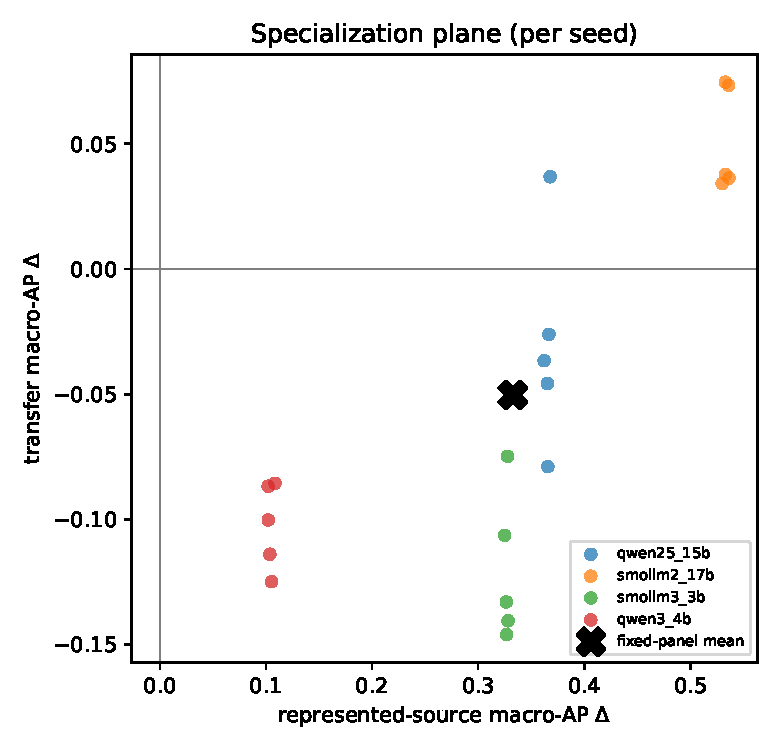
\includegraphics[width=0.94\columnwidth]{figures/specialization_plane.pdf}
\caption{Specialization plane. Each point is one (checkpoint, seed): horizontal axis is represented-source macro-AP change and vertical axis is transfer macro-AP change. Fourteen of twenty seeds lie in the lower-right specialization quadrant; six lie in uniform gain---all five SmolLM2-1.7B seeds and Qwen2.5-1.5B seed 43. The fixed-panel observed point is shown separately.}
\Description{Scatter plot of twenty seed-level base-to-SFT changes. All points have positive represented-source change; fourteen have negative transfer change and six have positive transfer change. The fixed-panel mean lies in the specialization quadrant.}
\label{fig:plane}
\end{figure}

\section{Limitations}
\label{sec:limitations}

We frame this as a controlled measurement study, and several caveats bound its interpretation.

\textbf{Heterogeneous native policies.} The transfer benchmarks encode different native label constructs (harm, refusal, jailbreak, contrast), so their macro-average mixes distinct policies rather than measuring one fixed policy.

\textbf{Fixed two-lineage panel.} The panel is four purposively chosen checkpoints spanning two model lineages (Qwen and SmolLM); the estimand is this panel, and results do not extrapolate to other architectures, scales, or vendors.

\textbf{Previously inspected benchmarks.} The public or gated benchmark datasets have been examined during pipeline development, so they are held out from SFT but were not prospectively unseen during development; measured transfer is dataset-held-out, not a guarantee against distributional familiarity.

\textbf{Retrospective legacy artifact.} The committed lock predates the strengthened code/artifact contract and records a dirty source tree. WildGuardTest and WildJailbreak use frozen seed-7 cohorts rather than the corrected pinned-source hash selection. Local HPO code and logs show that the frozen-cache evaluation pathway was repeatedly scored during development, although the optimization objective used represented-source development AP; the logs do not fingerprint the cache bytes. This creates adaptive-exposure risk even though the final SFT loss did not consume transfer rows. Rebuilding by the declared hash rule replaces 605 of the 1{,}220 WildGuard/WildJailbreak cohort rows but retains 615 previously inspected rows, so it repairs selection provenance without creating a genuinely untouched confirmatory set. The repaired pipeline invalidates the old lock; prospective confirmation requires a new uninspected cohort or benchmark.

\textbf{Family links and truncation.} The historical manifest failed to join 36 JailbreakBench matched-index pairs and 58 XSTest safe/unsafe pairs, and two represented-source families cross calibration and ID. In addition, 26 unique evaluation prompts were truncated (21--25 per checkpoint); nearly every truncated model rendering lost the full system instruction. Depending on the chat template, 16--17 training rows per checkpoint exceed the legacy prompt budget and are left-truncated, generally removing the system instruction. Corrected code preserves the family relationships and instruction, but only a new manifest, training run, and evaluation can replace the reported estimates.

\textbf{Balanced prevalence.} Represented-source and transfer test pools are near-balanced, whereas inline screening usually runs at much lower unsafe prevalence; precision, F1, and AP are prevalence-dependent, so balanced-set numbers overstate production precision at a fixed FPR.

\textbf{Non-commercial and gated data.} The study uses the non-commercial academic branch (ToxicChat is CC BY-NC 4.0) and gated AI2 sources (WildGuardMix, WildJailbreak), so redistribution is via identifiers, revisions, and hashes rather than raw text, and released adapters are non-commercial.

\textbf{Prompt-only scope.} The guard classifies input prompts only; response, tool-call, and full-dialogue moderation are out of scope and would require re-running the same discipline on those surfaces.

\textbf{Finite seeds and datasets.} Five training seeds per checkpoint and a small number of evaluation datasets bound statistical precision; the analysis reports seed-level values and leave-one-out sensitivities so readers can judge stability rather than treating the aggregate as a population estimate.

\section{Conclusion}
\label{sec:conclusion}

This paper estimates what one LoRA-SFT recipe changed relative to its untuned bases on a fixed four-checkpoint panel. In the legacy artifact, the observed represented-source change is $\RepDelta$ and the observed dataset-held-out transfer change is $\TransferDelta$; all leave-one-checkpoint-out and leave-one-transfer-benchmark-out transfer estimates remain negative. The per-checkpoint effects are heterogeneous, one checkpoint improves on transfer, and HarmBench recall falls substantially. These facts support an estimation-only description of \emph{in-source specialization on this panel}, not a universal claim that fine-tuning harms transfer or a confirmatory rejection.

The practical takeaway survives the narrower wording: evaluate an adapted guard against its own base on represented sources, dataset-held-out benchmarks, and safety/over-refusal stress sets. The corrected fail-closed pipeline makes the remaining evidentiary boundary explicit: a new manifest, training run, and scoring run are required before this panel-limited result can be promoted from legacy-artifact status to a clean-run result.

\appendix

\section{Provenance and Statistical Appendix}
\label{app:provenance}

The release separates two artifact contracts. The historical \texttt{LOCK.json}, row-keyed score table, score metadata, run metadata, and analysis outputs reproduce the legacy estimates only when the explicit legacy flag is supplied. New locks are self-hashed and bind the configuration, every manifest, audit, text-free public release, prompt rendering, source state, and expected score schema/code version. Score metadata then binds the lock, adapters/manifests, cache-producer runtime, batch size, and score-file digest; analysis rejoins score identities to locked manifests and revalidates adapters, calibration, thresholds, and predictions before reading the matrix. Training, evaluation, and analysis fail closed on missing or mismatched inputs. A separate recursively redacted public-manifest directory exposes identifiers, revisions, hashes, family links, license evidence, selection provenance, and counts without raw or normalized prompt text. The analysis emits deterministic \texttt{results.json}, runtime/source attestation in \texttt{analysis\_metadata.json}, descriptive \texttt{claim\_checks.json}, \texttt{seed\_values.csv}, \texttt{per\_benchmark.csv}, \texttt{sensitivity.json}, generated tables, and the specialization-plane figure. The main-text table and figure copies are verified byte-for-byte during the paper build.

\begin{table*}[t]
\centering
\small
\caption{Observed represented-source and transfer macro-AP changes for every legacy SFT seed. This table is generated from the same validated score matrix as \Cref{tab:primary}.}
\label{tab:seed-values}
\input{tab_seed_values_gen}
\end{table*}
\FloatBarrier

\section{Optional External Validation: ExpGuard}
\label{app:external}

The expert-annotated specialized-domain moderation benchmark ExpGuard \cite{expguard2026} provides a differently sourced prompt-moderation set (finance, healthcare, law) and is a natural replication target. Re-running the paired base-versus-SFT comparison on ExpGuard with a prospectively locked protocol would test whether the observed represented/transfer pattern recurs on an external expert-labeled source. We report no ExpGuard result here.

\bibliographystyle{ACM-Reference-Format}
\bibliography{refs}

\end{document}
